\chapter{Reverse Engineering}

L'ingegneria inversa si può definire in maniera precisa come quel processo 
in cui andiamo ad \textit{analizzare un sistema per creare rappresentazioni
ad alto livello di astrazione.}

\subsubsection{Cosa significa?}

Immaginiamo di essere \textit{Ferrari} e di voler realizzare un motore; partiremmo da
delle specifiche di massima sulla base delle quali svilupperemo un progetto.
Man mano il progetto includerà ad esempio i disegni delle componenenti meccaniche, 
le indicazioni su come assemblarle \dots

Tutte queste informazioni saranno poi mandate ad un impianto di produzione che 
andrà a comporre il motore; questo è il normale \textit{processo ingegneristico}.

Nell'\textbf{ingegneria inversa} vogliamo fare il contrario: partire da un \textit{prodotto finito} e 
e ricavare le \textit{informazioni progettuali}.

\begin{figure}[ht]
    \centering
    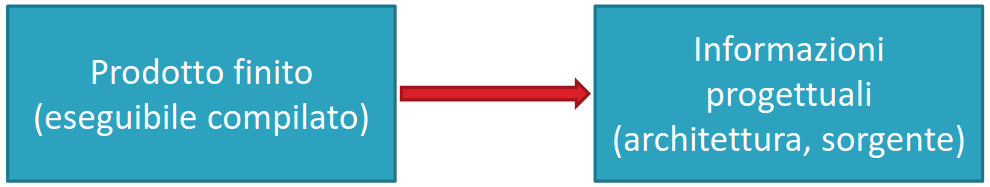
\includegraphics[width=0.75\linewidth]{images/reverse.png}
\end{figure}

Quando caliamo questo processo nel \textit{software reverse engineering}, il prodotto
finito è solitamente un \textbf{eseguibile compilato}; ciò che noi vogliamo ricavare sono delle
informazioni come ad esempio:
\begin{itemize}
    \item architettura del programma
    \item come funziona internamente (ad esempio certi algoritmi)
    \item completo recupero del codice del programma (caso estremo, in genere è sufficiente ricavare certe informazioni)
\end{itemize}

\subsubsection{Perché si fa reverse engineering?}

Esistono molte ragioni per fare \textit{reversing:}
\begin{itemize}
    \item un'azienda che produce un software e perde parti del codice sorgente,
    ha bisogno di \textbf{recuperare codice} per evitare perdite
    \item devo interagire con un sistema la cui \textbf{documentazione è mancante o insufficiente}
    \item \textbf{analisi dei prodotti dei concorrenti} nell'ambito industriale
    \item \textbf{"aprire" delle piattaforme proprietarie,} come ad esempio le console dei videogiochi
    \item \textbf{auditing di sicurezza:} ho un eseguibile ma non ho il codice sorgente, e voglio 
    analizzarlo per cercare delle vulnerabilità di sicurezza
    \item \textbf{\textit{curiosità}}
\end{itemize}

\section{La vita di un programma}

\subsubsection{Perché è difficile fare analizzare un binario compilato?}

Perché nel codice sorgente ci sono una serie di informazioni ad alto livello utili
per aiutare l'uomo a comprendere il software (nomi delle variabili, funzioni, commenti \dots),
ma che sono inutili per la macchina; nella fase di \textbf{compilazione} queste informazioni
vengono scartate. 

Avviene anche una traduzione dai linguaggi ad \textit{alto livello} in \textbf{codice macchina},
comprensibile ed eseguibile dalla macchina; questo codice è progettato per essere eseguibile dalla macchina,
non per essere facilmente comprensibile da un umano.

\begin{figure}[ht]
    \centering
    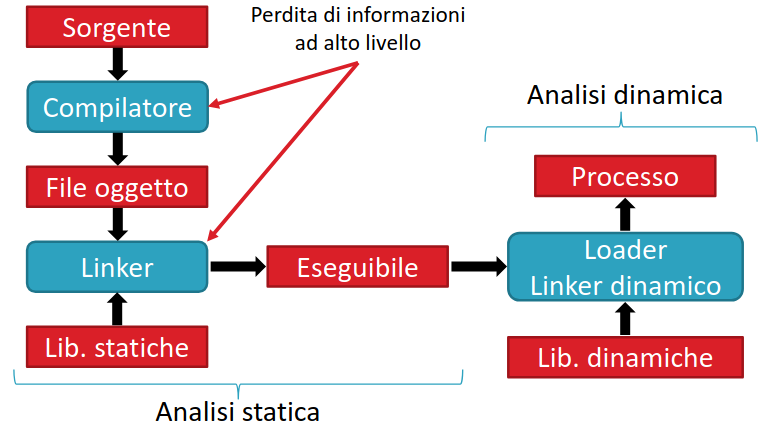
\includegraphics[width=0.75\linewidth]{images/program-life.png}
    \caption{Vita di un programma}
\end{figure}

Nel reversing distinguiamo due tipi principali di \textit{analisi}, che corrispondono alle due fasi della vita di un programma.

Dopo la fase di compilazione otteniamo un \textbf{\textit{file eseguibile}}; analizzare tale file (codice, dati, \dots) senza eseguirlo 
prende il nome di \textbf{analisi statica}.

Diversamente, un eseguibile può diventare un \textbf{\textit{processo}}; studiare il programma
mentre esegue (ad esempio un debugger) prende il nome di \textbf{analisi dinamica}.

\section{Eseguibili}

Esistono molti formati di eseguibili a seconda del sistema operativo; noi ci 
focalizziamo su \textbf{ELF} (\textit{Executable Linking Format}), il formato dell'ambiente Linux.

In generale, i concetti di base sono gli stessi per tutti i formati: ogni eseguibile definisce una serie
di \textbf{sezioni} o \textbf{segmenti} che sono delle parti del programma che saranno mappate in memoria
virtuale a \textit{runtime}. Ad esempio, potremmo avere:
\begin{itemize}
    \item un segmento per il codice macchina
    \item un segmento per i dati, a loro volta divisi in:
    \begin{itemize}
        \item un segmento per i dati \textit{read-only}
        \item un segmento per i dati scrivibili
    \end{itemize}
\end{itemize}
Vengono usati segmenti diversi per permettere di mapparli in aree di memoria virtuale
con \textbf{permessi diversi}.

\section{Gli strumenti}

\subsection{Analisi statica}

\begin{itemize}
    \item \textbf{Disassemblatore:} il linguaggio macchina grezzo è estremamente difficile da leggere; con esso 
    viene tradotto nel linguaggio \textbf{\textit{assembly}}, il quale permette di facilitare
    la comprensione
    \item \textbf{Decompilatore:} partendo dall'assembly cerca di \textbf{ricostruire il codice 
    sorgente del programma} (in un linguaggio \textit{simil-C}); spesso la ricostruzione non è 
    fedelissima per svariate ragioni (si perdono nomi delle variabili/funzioni, alcune strutture di controllo ad alto livello 
    vengono ottimizzate dal compilatore facendolo apparire diversamente nel codice macchina, \dots), ma 
    sono comunque uno strumento molto utile
\end{itemize}
\textit{Ghidra} è un tool di reversing che integra entrambi questi strumenti.

Un'altro strumento avanzato è \textit{Anger}, il quale effettua un'\textbf{esecuzione simbolica}: ogni
istruzione del programma viene trasformata in dei vincoli logici per rispondere alla domanda
\textit{"che input devo dare al programma per far sì che arrivi in un certo punto con
un certo stato?"}.


\subsection{Analisi dinamica}

\begin{itemize}
    \item \textbf{Debugger:} sono in grado di lavorare su file binari (eseguibili senza sorgente);
    un esempio è \textit{GDB}. Permette di studiare l'evoluzione del programma durante la sua esecuzione
    \item \textbf{instrumentazione dinamica:} è una tecnica che permette di iniettare del codice
    che verrà eseguito in risposta a determinati eventi; un tool è \textit{Frida} 
\end{itemize}

\section{Assembly x86\_64 (64 bit)}

Il processore non lavora direttamente sulla memoria, ma su una piccola memoria locale
contenente una serie di variabili dette \textbf{registri}. Questo viene fatto perché la
RAM è \textbf{molto lenta} (per il processore), mentre i registri essendo una memoria molto piccola
riescono a girare alla sua stessa velocità; dalla memoria dunque le informazioni
necessarie vengono caricate nei registri.

Ogni istruzione assembly ha:
\begin{itemize}
    \item uno \textbf{mnemonico} che indica ciò che quell'istruzione fa (ad esempio \texttt{add} per l'addizione)
    \item degli \textbf{operandi}, che possono essere dei registri o delle locazioni di memoria, che 
    indicano i dati su cui opera l'istruzione
\end{itemize}
Notazione \textit{Intel}: \texttt{<op> <destinazione>, <sorgente>}

Ad esempio: \texttt{add r1, r2}

\subsection{Registri x86\_64}

Ha dei registri che sono l'estensione a 64 bit di alcuni 
registri di x86 (a 32 bit), con il nome di: \texttt{rax, rbx, rcx, rdx}

Ci sono alcuni registri speciali:
\begin{itemize}
    \item \texttt{rip:} sta per \textit{instruction pointer}, è il registro che prende
    \textbf{l'indirizzo dell'istruzione corrente}; prende anche il nome di \textbf{program counter}
    \item registri per la \textbf{gestione dello stack}:
    \begin{itemize}
        \item \texttt{rsp}: è lo \textbf{stack pointer}, punta alla cima dello stack
        \item \texttt{rbp}: è il \textbf{frame pointer}, è utilizzato per tenere traccia della porzione 
        di stack che contiene le variabili locali della funzione corrente 
    \end{itemize}
\end{itemize}

Sono infine presenti dei \textbf{registri generici}, nominati da \texttt{r8} a \texttt{r15}.

\subsubsection{La struttura dei registri}

I registri x86\_64 sono un po' \textit{complicati}, in quanto presentano una forma a matriosca,
mostrata in Figura \ref{fig:regx86}.

\begin{figure}[ht]
    \centering
    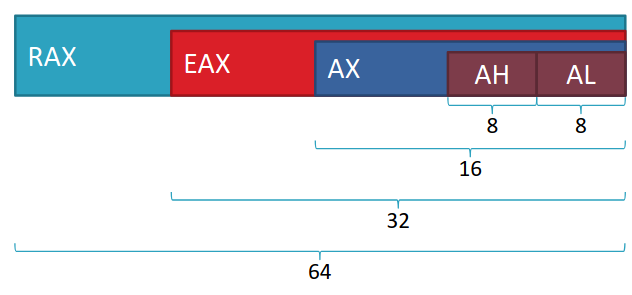
\includegraphics[width=0.75\linewidth]{images/registri.png}
    \caption{Registri x86}
    \label{fig:regx86}
\end{figure}

Quando x86 era a 16 bit, c'era il registro \texttt{ax} (oppure \texttt{bx, \dots}); era possibile
accedere agli 8 bit \textit{alti} o \textit{bassi} utilizzando i registri \texttt{ah} (\textit{high}) o \texttt{al} (\textit{low}).

Quando è stato introdotto x86 a 32 bit, si voleva mantenere compatibilità con le applicazione a 16 bit;
è stato quindi introdotto un registro \texttt{eax} (\textit{extended} \texttt{ax}), mantenendo
quello che prima era \texttt{ax} come la metà bassa del nuovo registro a 32 bit.

Quando è stato introdotto x86 a 64 bit, per mantenere nuovamente la compatibilità è stata fatta
la stessa cosa introducendo il registro \texttt{rax}, e tenendo il vecchio \texttt{eax} come 
i 32 bit bassi del nuovo registro a 64 bit.

Questo schema si applica anche ai registri \texttt{rbx, rcx, rdx}.

\subsection{Alcune istruzioni di base}

\begin{itemize}
    \item \texttt{MOV <dst>, <src> | MOV rax, rbx} $\rightarrow$ copia da una sorgente ad una destinazione
    \item \texttt{PUSH <src> / POP <dst>} $\rightarrow$ sono utilzzate per fare dei \textit{push/pop} sullo stack
    \item \texttt{ADD/SUB <dst>, <src>} $\rightarrow$ utilizzate per fare addizioni/sottrazioni
    \item \texttt{CALL <pc> / RET} $\rightarrow$ sono utilizzate per fare le chiamate a funzioni (\texttt{CALL}) o per
    ritornare da una istruzione al chiamante (\texttt{RET})
\end{itemize}

\newpage
\subsection{Salti condizionali}

Una feature fondamentale per un processore è essere in grado di prendere delle decisioni (come eseguire un \textit{statement} \texttt{if}); in 
assembly questo processo è diviso in due step:

\begin{enumerate}
    \item \texttt{CMP <op1> <op2>} $\rightarrow$ è una funzione che confronta i valori della condizione; successivamente, imposta
    alcune flag che descrivono l'esito del confronto
    \item \texttt{J <condizione> <pc>} $\rightarrow$ permette di \textbf{cambiare il progam counter saltando ad un'altra locazione del programma} se una certa flag
    di condizione è stata impostata
\end{enumerate}

Un \textit{loop} può essere implementato con un salto all'indietro, ovvero
salto all'inizio del loop finché la condizione non si falsifica.

\section{Reversing statico con Ghidra}

Abbiamo un piccolo binario, mostrato a destra in Figura \ref{fig:ex-ghidra1}, che chiede di inserire una chiave e risponde 
se è corretta o meno.

Facendo l'analisi con Ghidra possiamo ottenere le istruzioni assembly del binario; possiamo inoltre
attivare la vista del \textbf{control flow graph}, mostrato a sinistra in Figura \ref{fig:ex-ghidra1}.\\
Esso mostra il \textbf{flusso di esecuzione 
del programma:} ogni blocco è un insieme di istruzioni dette \textit{straight line}, cioè che non 
contengono salti (eccetto alla fine). Ogni blocco è collegato a quelli che possono essere 
i suoi successori.

\begin{figure}[ht]
    \centering
    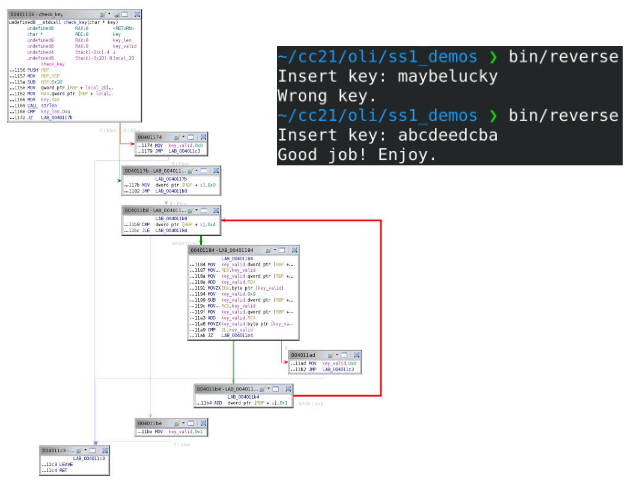
\includegraphics[width=1\linewidth]{images/static-ghidra1.png}
    \caption{Binario e Control Flow Graph}
    \label{fig:ex-ghidra1}
\end{figure}

Possiamo inoltre decompilare il binario ottenendo ciò che è mostrato
in Figura \ref{fig:ex-ghidra2} (rinominando le varabili).


\begin{figure}[ht]
    \centering
    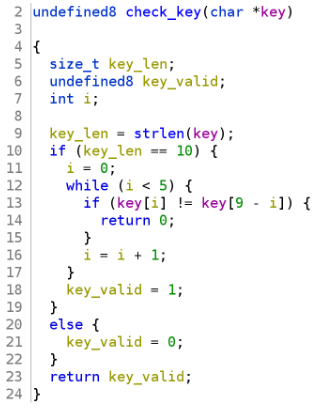
\includegraphics[width=0.5\linewidth]{images/static-ghidra2.png}
    \caption{Codice ottenuto attraverso la decompilazione e rinominando le variabili}
    \label{fig:ex-ghidra2}
\end{figure}





















